\subsubsection{Differenzverstärker}

\begin{figure}[H]
  \begin{center}
    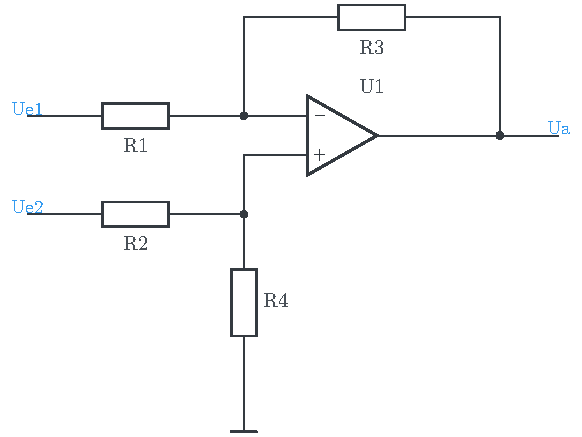
\includegraphics[width=0.618\textwidth]{circuits/differenz.pdf}
  \end{center}
  \caption{Differenzverstärkerschaltung}
\end{figure}

Der Differenzverstärker verstärkt die Differenz der Spannungen $U_{e1}$ und $U_{e2}$.

\begin{gather*}
  \intertext{Überlagerung:}
  U_a = U_a' + U_a''\\
  U_a' = U_a|_{U_{e2} = 0} = - U_{e1} \cdot \frac{R_3}{R_1}\\
  U_a'' = U_a|_{U_{e1} = 0} = U_p \cdot \left(1+\frac{R_3}{R_1}\right)\\
  = U_{e2}  \frac{R_4}{R_2 + R_4} \cdot \left(1+\frac{R_3}{R_1}\right)\\
  U_a = U_{e2}  \cdot \frac{R_4}{R_2 + R_4} \cdot \left(1+\frac{R_3}{R_1}\right) -
  U_{e1} \cdot \frac{R_3}{R_1}\\
  U_a = U_{e2}  \cdot \frac{R_4}{R_2 + R_4} + U_{e2} \cdot \frac{R_4}{R_2 + R_4}
  \cdot \frac{R_3}{R_1} - U_{e1} \cdot \frac{R_3}{R_1}
\end{gather*}
\noindent Wenn gilt $\frac{R_3}{R_1} = \frac{R_4}{R_2}:$
\eqbox{
  U_a = \frac{R_3}{R_1}\left(U_{e2} - U_{e1}\right)
}{0.382\textwidth}

\noindent Wenn alle Widerstände gleich dimensioniert werden:
\eqbox{
  U_a = U_{e2} - U_{e1}
}{0.382\textwidth}


\subsubsection{Instrumentationsverstärker}

\begin{figure}[H]
  \begin{center}
    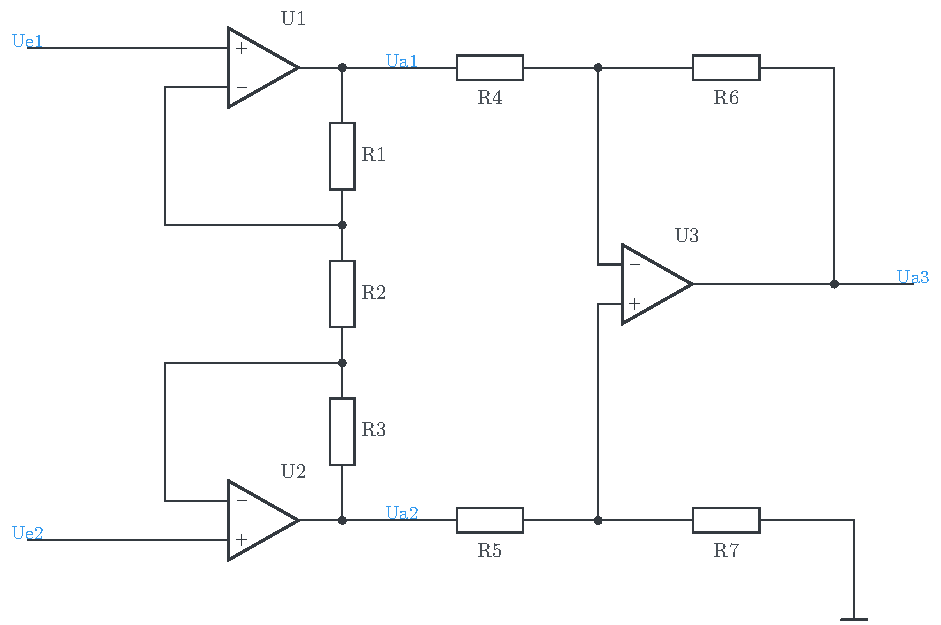
\includegraphics[height=0.618\textwidth]{circuits/instrument.pdf}
  \end{center}
  \caption{Instrumentationsverstärkerschaltung}
\end{figure}

\begin{gather*}
  \intertext{Virtuelle Masse, $U_d = 0$:}
  U_{R_2} = U_{e1} - U_{e2}\\
  I_{R_2} = \frac{U_{e1} - U_{e2}}{R_2}\\
  \intertext{für $I_n = 0$:}
  I_{R_1} = I_{R_2} = I_{R_3}\\
  U_{a1,2} = U_{a1} - U_{a2} = I_{R_3} (R_1 + R_2 + R_3)\\ 
  U_{a1} - U_{a2} = \frac{U_{e1}-U_{e2}}{R_2} (R_1 + R_2 + R_3)\\ 
  \intertext{für $R_1 = R_3$:}
  U_{a1} - U_{a2} = U_{e1} - U_{e2} \left( 1 + \frac{2 \cdot R_1}{R_2}\right)
\end{gather*}
  der Dritte OPV ist als Differenzverstärker geschaltet\\
  für $R_4 = R_5 = R_6 = R_7$ ist die Verstärkung $V_{OPV3} = -1$
    (Eingangsdifferenz tauschen)

\eqbox{
  U_{a3} = (U_{e2} - U_{e1}) \cdot (1 + \frac{2\cdot R_1}{R_2})
}{0.618\textwidth}
Die Verstärkung ist somit durch $R_2$ einstellbar
\subsubsection{Summierer}

\begin{figure}[H]
  \begin{center}
    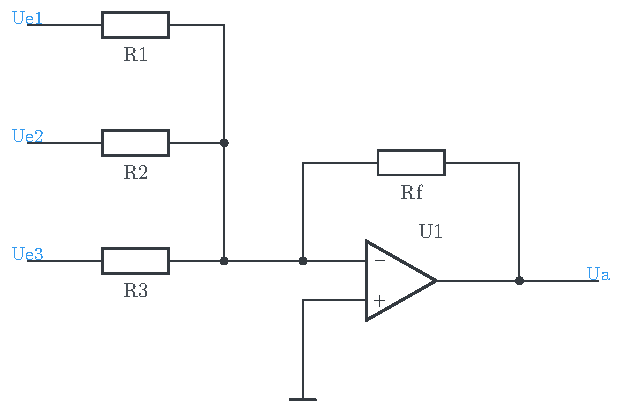
\includegraphics[width=0.618\textwidth]{circuits/summier.pdf}
  \end{center}
  \caption{Summierverstärkerschaltung}
\end{figure}

Der Summierverstärker verstärkt die Summe der gewichteten Eingangsspannungen.

\begin{gather*}
  I_{\mathrm{IN}} = \sum_{n=1}^N{I_{en}} = \frac{U_{e1}}{R_1}+
  \frac{U_{e2}}{R_2} + \cdots + \frac{U_{eN}}{R_N}\\
\end{gather*}
\eqbox{
  U_a = -\left( \frac{R_f}{R_1} U_{e1} + \frac{R_f}{R_2} U_{e2} + \cdots +
    \frac{R_f}{R_N} U_{eN} \right)
  }{0.618\textwidth+5mm}

\subsubsection{Integrator}
\begin{figure}[H]
  \begin{center}
    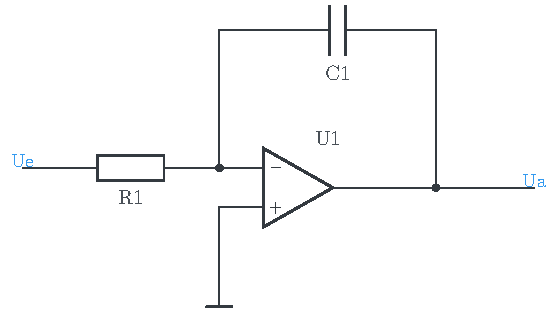
\includegraphics[width=0.618\textwidth]{circuits/integrier.pdf}
  \end{center}
  \caption{Integratorschaltung}
\end{figure}

\begin{gather*}
i_{R_1} = - i_{C_1}\\
\frac{u_e}{R_1} = - C_1 \cdot \frac{\dif u_a}{\dif t}
\end{gather*}
\eqbox{
u_a = - \frac{1}{R_1 C_1} \cdot \int{u_e \dif t}
}{0.382\textwidth}
Der Integrator bildet also das Integral der Eingangsspannung, wichtet es mit
$\frac{1}{RC}$ ($RC...\mathrm{Zeitkonstante}$) und invertiert es.

\subsubsection{Differentiator}
\begin{figure}[H]
  \begin{center}
    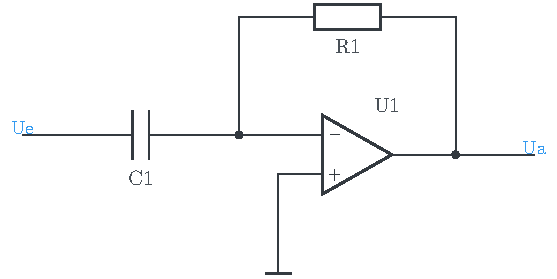
\includegraphics[width=0.618\textwidth]{circuits/differenzier.pdf}
  \end{center}
  \caption{Differentiatorschaltung}
\end{figure}

\begin{gather*}
i_{R_1} = - i_{C_1}\\
\frac{u_a}{R_1} = - C_1 \cdot \frac{\dif u_e}{\dif t}
\end{gather*}
\eqbox{
u_a = - {R_1 C_1} \cdot \frac{\dif u_e}{\dif t}
}{0.382\textwidth}
Der Differentiator differenziert die Eingangsspannung, wichtet das Ergebnis mit
$RC$ und invertiert es.
